\documentclass{article}
\usepackage[utf8]{inputenc}
\usepackage[french]{babel}
\usepackage{float} % Ajoute ce package pour utiliser l'option H
\usepackage{graphicx}

\title{Rapport : Agents Intelligents}
\author{Alexandre Faure, Valentin Cuzin-Rambaud}
\date{\today}

\begin{document}

\maketitle

\section{Introduction}

\subsection{Rappel et choix du sujet}

Dans le cadre de ce projet, nous avons choisi de travailler sur le thème des robots explorant une planète lointaine dans le but de collecter des pierres rares. Ce sujet s'inscrit dans le contexte des agents intelligents, et en particulier des agents BDI (Belief-Desire-Intention). Nous utilisons la plateforme JADE (Java Agent Development Framework) pour simuler et gérer l'interaction des agents dans cet environnement complexe.

L’objectif des agents, dans cet exemple inspiré des travaux de Steels, est de localiser et de récupérer des pierres rares disséminées sur une planète inexplorée et difficile d'accès. Les agents n'ont pas de carte de cette planète, dont le terrain est très accidenté, et ils doivent être capables de naviguer de manière autonome. De plus, une fois leur mission accomplie, les robots doivent pouvoir retourner au vaisseau spatial en utilisant un signal émis continuellement, dont l’intensité les aide à se repérer.

Dans ce rapport, nous allons détailler les choix techniques et conceptuels liés à la conception de ces agents explorateurs, en insistant particulièrement sur leur architecture BDI et sur l'utilisation de JADE pour leur développement.

\section{Choix de consception}

\subsection{L'environnement}

Dans notre simulation, la planète est représentée par un tableau de cases, où chaque case représente une portion de terrain avec ses spécificités, comme par exemple son niveau de difficulté pour être parcourue et explorée. Chaque case a également une probabilité de contenir des pierres rares, ou bien d'être totalement infranchissable pour un robot. 

Comme précisé dans l'énoncé, lorsqu'une case contient des pierres rares, celles-ci sont regroupées en tas, et leur nombre se situe entre 5 et 10. Pour collecter ces pierres, le robot doit d'abord fouiller la case afin de les localiser. Pour se déplacer d'une case à l'autre, le robot doit prendre en compte le temps nécessaire pour traverser la case, qui dépend de son niveau de difficulté.

La planète contient plusieurs types de pierres, chacune ayant une rareté et une valeur différentes. Pour notre simulation, nous avons inclus des pierres de types "diamant", "rubis", "émeraude", "saphir" et "autre". Lorsqu'un robot collecte des pierres, celles-ci occupent un certain espace de stockage. Lorsque cet espace est plein, le robot décide de retourner au vaisseau pour vider son chargement. Avant de partir, s'il reste des pierres sur la case, le robot envoie un message aux autres robots pour indiquer la présence de pierres à ces coordonnées. Ainsi, si un autre robot se trouve à proximité, il pourra s'y rendre pour les collecter.

Au centre de la planète se trouve le vaisseau, qui communique en permanence avec les robots en émettant un signal pour les guider vers lui. Lorsqu'un robot envoie un signal pour stocker ses pierres, le vaisseau reçoit le chargement et stocke les pierres.

\begin{figure}[H]
    \begin{minipage}{\textwidth}
        \centering
        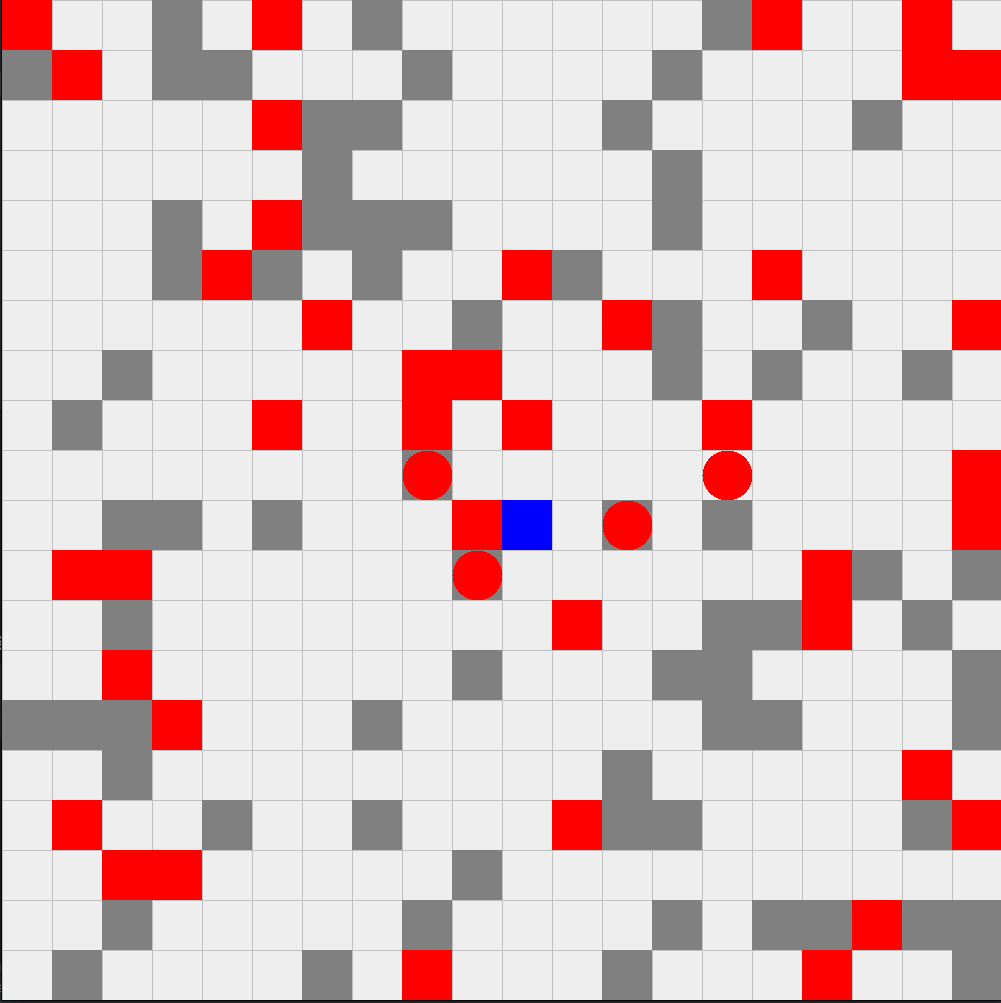
\includegraphics[scale=0.35]{./img/env1.png}
        \caption{Capture d'écran de l'interface graphique de la simulation}
        \label{fig:ResAg1}
    \end{minipage}
\end{figure}

Sur la Figure~\ref{fig:ResAg1}, on peut observer l'environnement dans son ensemble, représenté sous forme de grille. Les cases en rouge sont les cases dites "infranchissables", les cases en gris contiennent des pierres, et les cercles rouges (ici au nombre de quatre) représentent les robots qui explorent la planète. La case bleue indique la position du vaisseau.

\begin{figure}[H]
    \begin{minipage}{\textwidth}
        \centering
        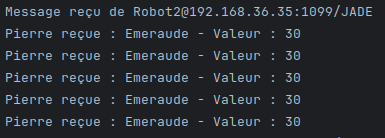
\includegraphics[scale=0.35]{./img/com_R-S.png}
        \caption{Capture d'écran de la communication entre un robot et le vaisseau pour déposer des pierres}
        \label{fig:ResAg2}
    \end{minipage}
\end{figure}

\begin{figure}[H]
    \begin{minipage}{\textwidth}
        \centering
        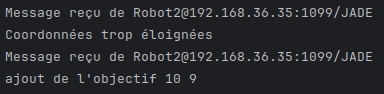
\includegraphics[scale=0.35]{./img/com_R-R.png}
        \caption{Capture d'écran de la communication entre deux robots pour signaler la présence de pierres}
        \label{fig:ResAg3}
    \end{minipage}
\end{figure}



\end{document}
